
\documentclass[12pt,onecolumn]{scrartcl}
\usepackage[margin=0.9in]{geometry}
%\usepackage{mhchem} % Package for chemical equation typesetting
%\usepackage{siunitx} % Provides the \SI{}{} command for typesetting SI units
%\usepackage[T2A]{fontenc}
%\usepackage[cp1251]{inputenc}
%\usepackage[english,russian]{babel}
%\usepackage{indentfirst}
%\usepackage{enumerate}
\usepackage{texshade}
\usepackage{subfig}
\usepackage{graphicx} % Required for the inclusion of images

%\usepackage{morefloats}

%\usepackage{wrapfig}
%\usepackage{lscape}
%\usepackage{rotating}
\usepackage{hyperref}
\usepackage{lscape}
\hypersetup{colorlinks=true,urlcolor=blue}
\urlstyle{same}



%\setlength\parindent{30pt} % Removes all indentation from paragraphs

%\renewcommand{\labelenumi}{\alph{enumi}.} % Make numbering in the enumerate environment by letter rather than number (e.g. section 6)

\usepackage{times} % Uncomment to use the Times New Roman font

%----------------------------------------------------------------------------------------
%	DOCUMENT INFORMATION
%----------------------------------------------------------------------------------------

\title{Nucleosome LEGO} % Title
\subtitle{\url{https://github.com/molsim/nuclLEGO} \\ Model variant 1: DNA and histone dimers }


\author{by \\ Alexey Shaytan \footnote{alexey.shaytan at gmail dot com}} % Author name

\date{\small{\today}} % Date for the report

\begin{document}

\maketitle % Insert the title, author and date


% If you wish to include an abstract, uncomment the lines below
%\begin{abstract}

%\end{abstract}
%----------------------------------------------------------------------------------------
%	BODY
%----------------------------------------------------------------------------------------

\section{Model description}
The model is based on X-ray structure of nucleosome core particle from \textit{Xenopus laevis} histones and $\alpha$-satellite DNA sequence (PDB ID: 1KX5, Davey et al. 2002). Flexible histone tails we truncate and only following parts of histone sequence were retained in the model: H3 (45-end), H4 (24-end), H2A (15-118), H2B (30-end). Suggested color coding is seen in Figure \ref{colorcode}.

\begin{figure}[h]
\begin{center}
\subfloat{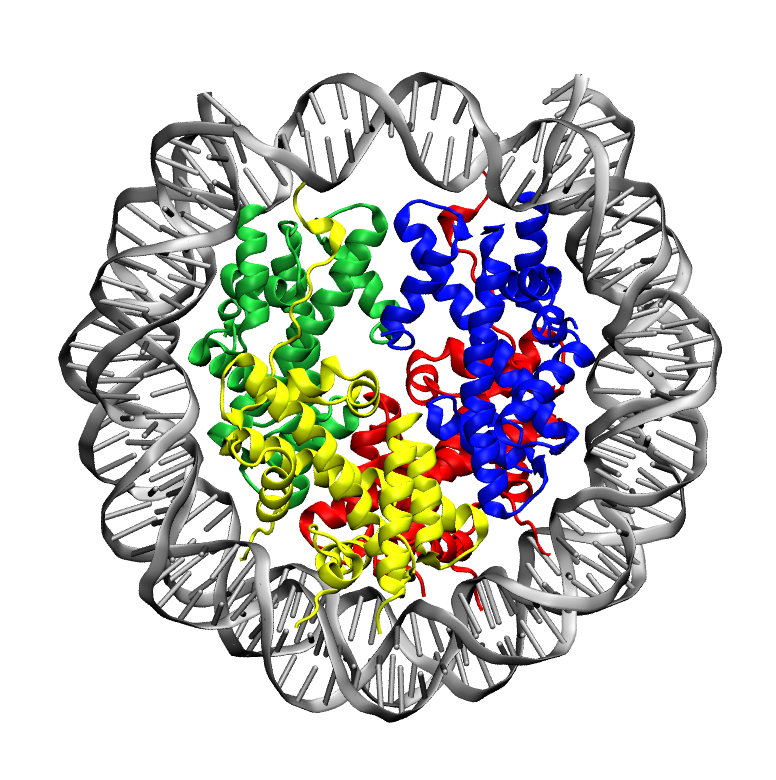
\includegraphics[width=0.5\textwidth]{img/nucl_ss} }
\subfloat{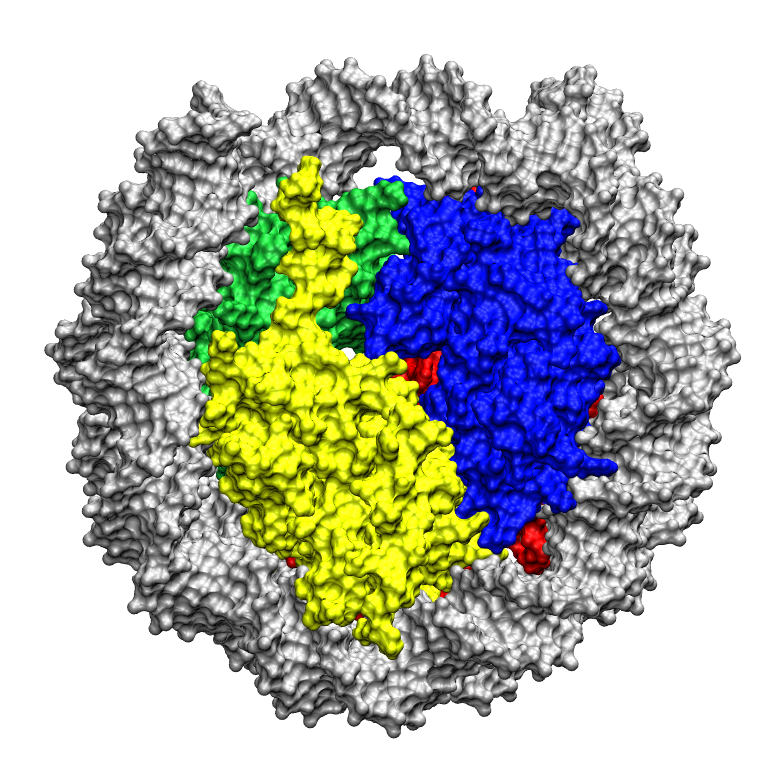
\includegraphics[width=0.5\textwidth]{img/nucl_surf}}
\caption{Suggested color coding of nucleosome parts: first H3-H4 dimer (chains A,B) - blue, second H3-H4 dimer (chains E,F) - green, first H2A-H2B dimer (chains C,D) - yellow, second H2A-H2B dimer (chains G,H) - red, DNA (chains I,J) - white/grey.}
\label{colorcode}
\end{center}
\end{figure}

\section{Assembly instructions}
See video at \url{http://youtu.be/BVYtnfIcnH4}
\begin{itemize}
\item Locate histone dimers and their key binding elements (Figure \ref{dim_elem}). For H3-H4 - 4-helix bundle site of H3 histone with bidentate protrusion of LYS115 and HIS113, 4-helix bundle site of H4 histone with bidentate protrusion of LYS77 and HIS75, H4 TYR98 at C-terminal $\beta$-sheet. For H2A-H2B dimer - H2B 4-helix bundle site and ARG89, H2A docking domain.
\item Locate DNA. DNA sequence is symmetric except for the central AT base pair. Locate the additional methyl group of central T protruding from the major groove DNA surface. This methyl group pinpoints the 'upper side' of nucleosome. (Figure \ref{dna})
\item Attache two H3-H4 dimers (blue and green) to each other via 4-helix bundle interaction.
\item Take yellow H2A-H2B dimer, insert ARG89 between H4LYS77 and H4HIS75 of blue H3-H4 dimer and attach H2A-H2B dimer by guiding the docking domain into its natural position, pay attention to H4TYR98 of the green dimer which should fit into cavity on the yellow H2A-H2B surface.
\item Do the same with the red H2A-H2B dimer, check the interaction of two H2A-H2B dimers at the dyad axis with L1 loops.
\item Locate the 14 arginines at the surface of the octamer, which should be inserted into minor grooves of nucleosomal DNA. See Figure \ref{14arginines}. These arginines are at superhelix locations (SHL) $\pm0.5,\pm1.5,\pm2.5,\pm3.5,\pm4.5,\pm5.5,\pm6.5$
\item Orient DNA so that thymine of the central base pair is closer to the blue H3-H4 dimer, locate the two symmetric minor grooves of DNA nearest to the DNA central base pair, locate two symmetric H4 arginines that should fit into these minor grooves.
\item Gently but uniformly push the ends of nucleosomal DNA along the DNA path, so that the DNA superhelix will uniformly deform and its radius will increase to enable the DNA pass through the top of nucleosome into its position on the octamer.
\item Put the DNA onto the octamer by first allowing the H4 arginines fit into the symmetric minor grooves. At this loin arginines at SHL $\pm1.5,\pm2.5$ should also be in place.
\item Now we need to get all other key arginines in place to their minor grooves at corresponding SHL. The idea is to pull DNA carefully but sufficiently strong at the corresponding SHL and consecutively put all the key arginines into minor grooves. It is important to apply force to DNA without applying to much pressure to the arginines, since they might break away (especially H2BARG30). In case the arginines break away they can be easily glued back with super glue.
\end{itemize}

\begin{figure}[h]
\begin{center}
\subfloat{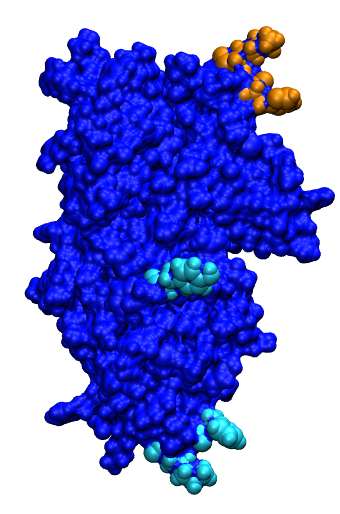
\includegraphics[width=0.35\textwidth]{img/h3h4} }
\subfloat{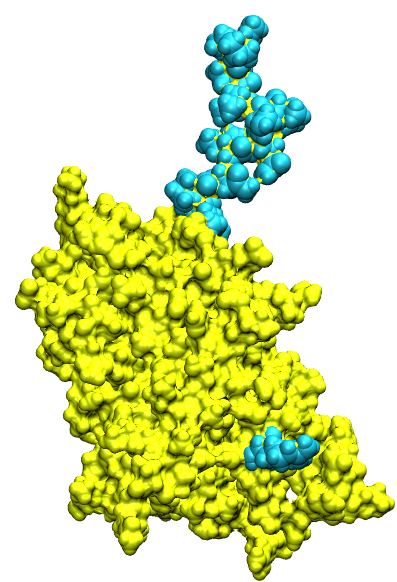
\includegraphics[width=0.35\textwidth]{img/h2ah2b}}
\caption{Anchor elements in H3-H4 (left) and H2A-H2B (right) dimers. H3 4-helix bundle site - orange, H4 4-helix bundle site and TYR98 - cyan, H2A - docking domain and H2B 4-helix bundle site - cyan.}
\label{dim_elem}
\end{center}
\end{figure}

\begin{figure}[h]
\begin{center}
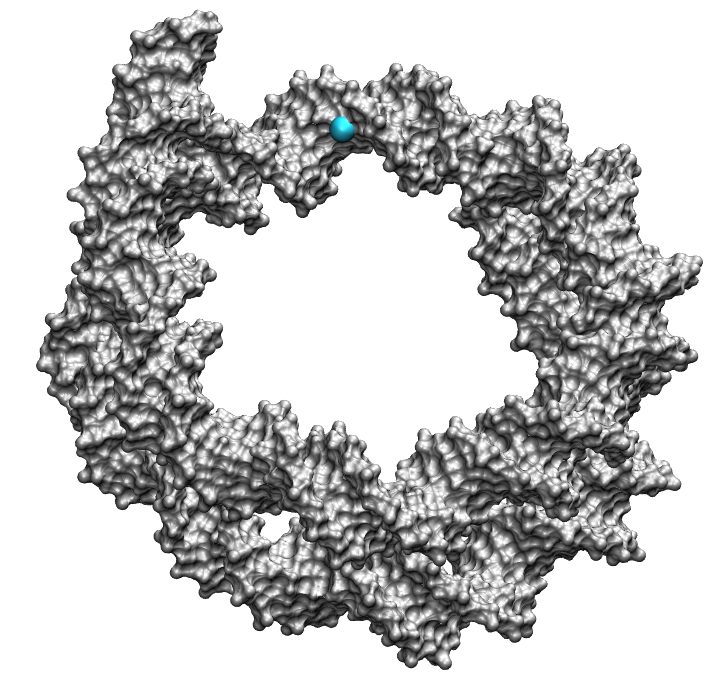
\includegraphics[width=0.7\textwidth]{img/dna} 
\caption{Anchor elements in DNA: the methyl of thymine in central base pair depicted in cyan.}
\label{dna}
\end{center}
\end{figure}

\begin{figure}[h]
\begin{center}
\subfloat{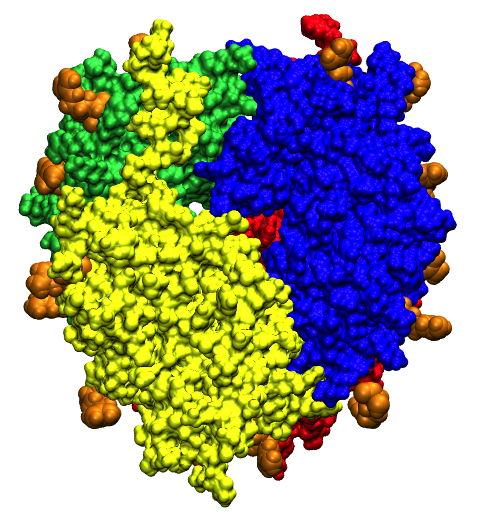
\includegraphics[width=0.25\textwidth]{img/arg1} }
\subfloat{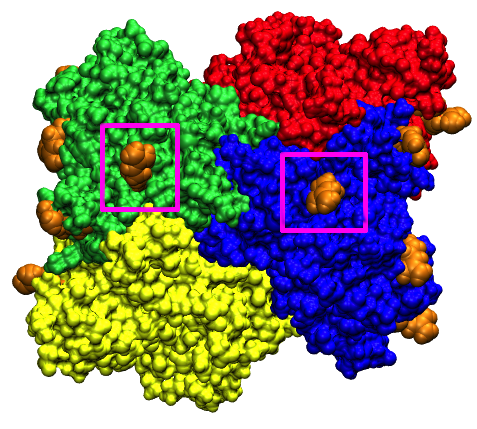
\includegraphics[width=0.25\textwidth]{img/arg2} }
\subfloat{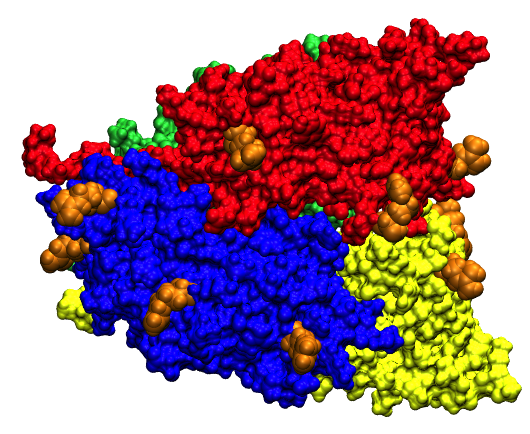
\includegraphics[width=0.25\textwidth]{img/arg3} }
\subfloat{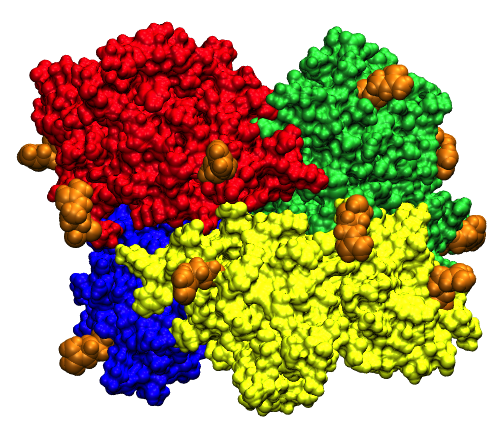
\includegraphics[width=0.25\textwidth]{img/arg4} }
\caption{14 key arginines residing in DNA minor grooves on the surface of histone octamer depicted in orane. Arginines at SHL $\pm0.5$ highlighted by magenta boxes.}
\label{14arginines}
\end{center}
\end{figure}

\section{Final model pictures}
Initial parts in Figure \ref{parts} and assembled model in Figure \ref{nucl}.

\begin{figure}[h]
\begin{center}
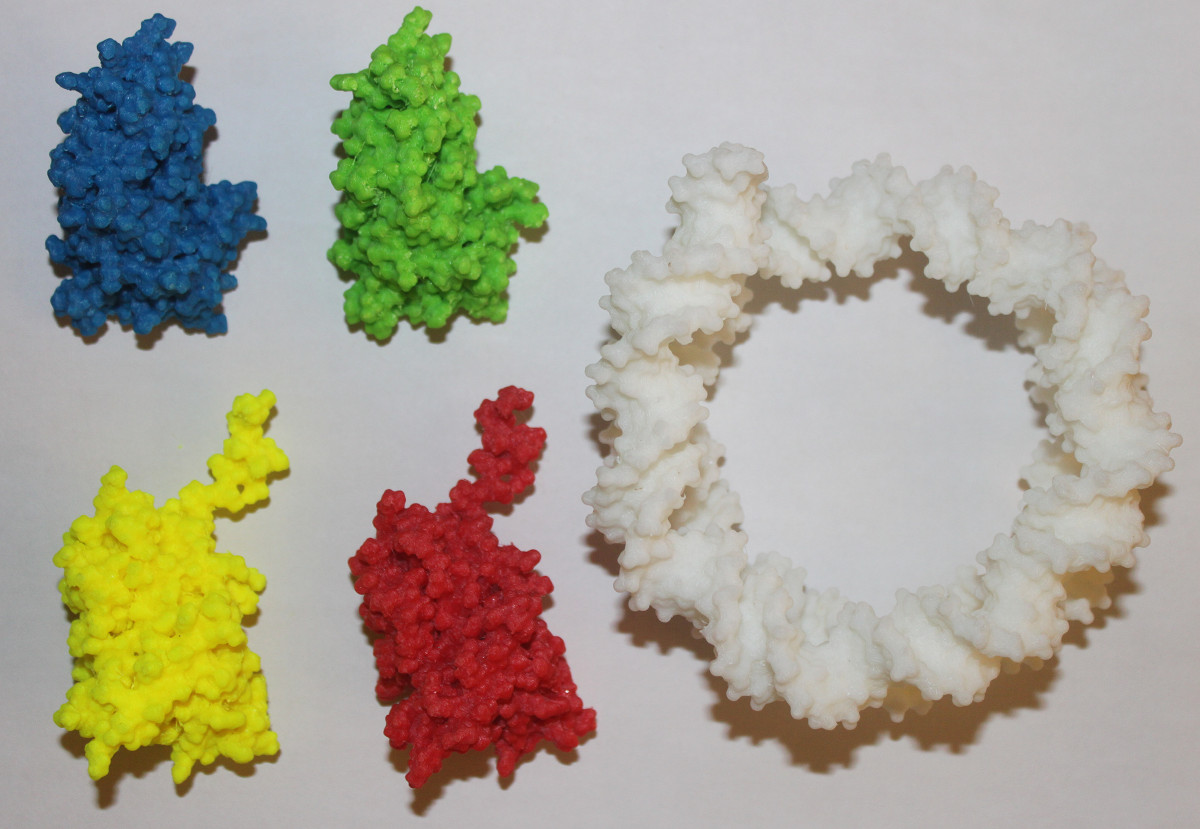
\includegraphics[width=1.0\textwidth]{img/nucl_parts} 
\caption{Plastic parts of nucleosome assembly kit.}
\label{parts}
\end{center}
\end{figure}

\begin{figure}[h]
\begin{center}
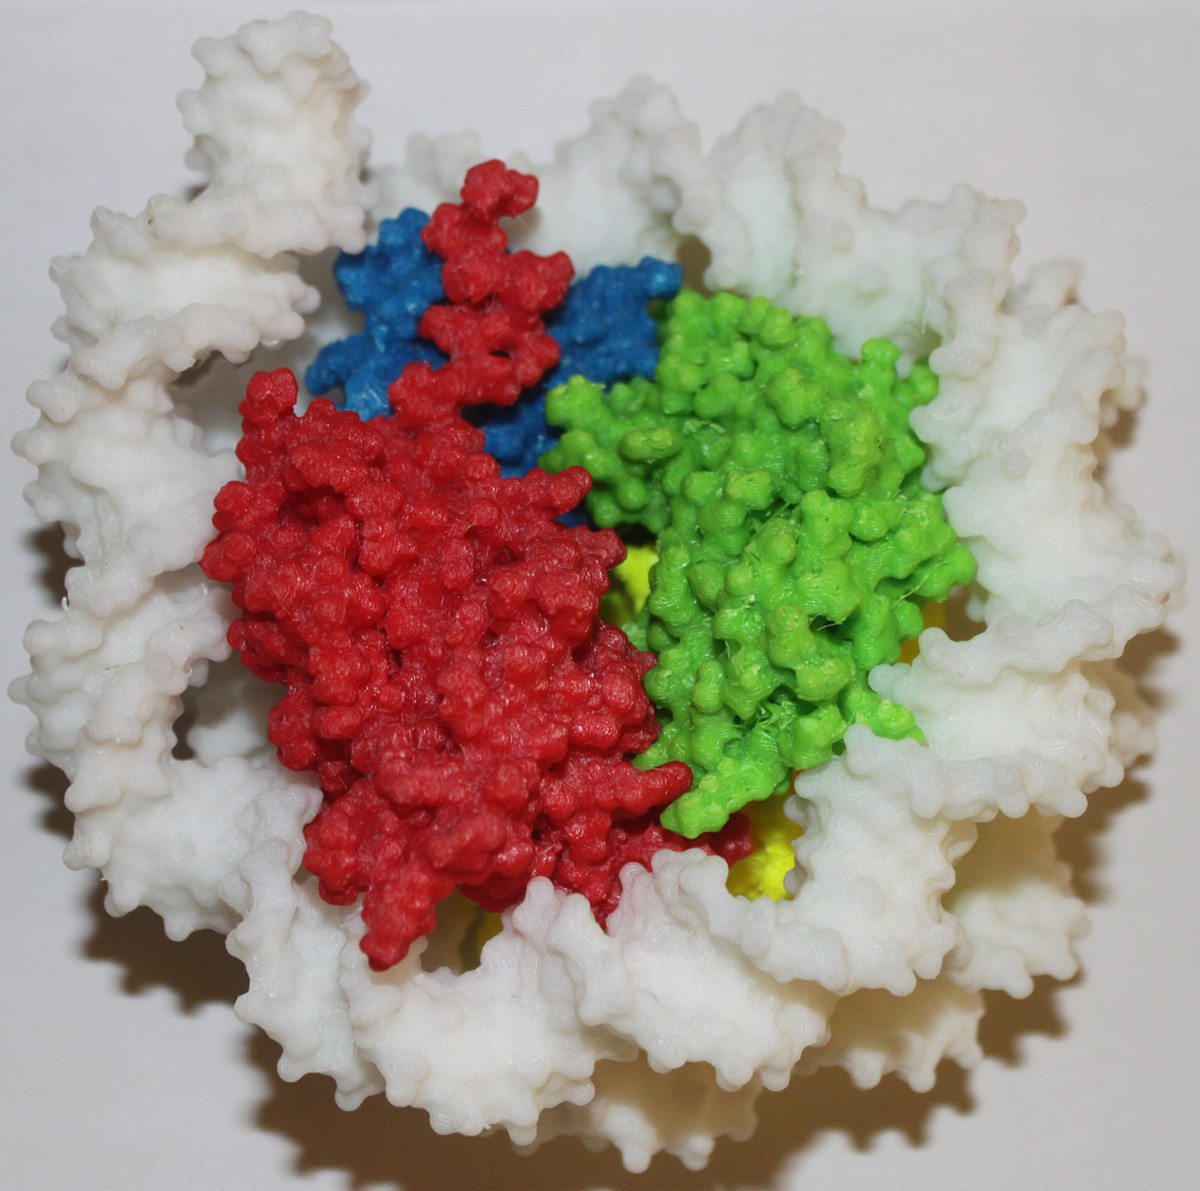
\includegraphics[width=1.0\textwidth]{img/nucl} 
\caption{Assembled plastic model of nucleosome core particle.}
\label{nucl}
\end{center}
\end{figure}

\section{Final notes}
Please, send your comments and suggestions at alexey.shaytan at gmail dot com.

\begin{landscape}
\section{Appendix A: Histone sequences}


\begin{texshade}{seq/h3.fasta}

\residuesperline*{80}
        
%\threshold[5]{1}
\shadeallresidues
\shadingmode[hydropathy]{functional}
\showruler{top}{1}
\ttopspace{-\baselineskip}
\hideconsensus
\defconsensus{{}}{*}{upper}
\hideseq{dum}

\feature{top}{consensus}{85..114}{helix}{alpha2}\feature{top}{consensus}{120..131}{helix}{alpha3}\feature{top}{consensus}{63..77}{helix}{alpha1}\frameblock{consensus}{83..83}{Red[1.5pt]}\frameblock{consensus}{49..49}{Red[1.5pt]}\frameblock{consensus}{63..63}{Red[1.5pt]}\feature{tttop}{consensus}{78..84}{loop}{loopL1}\feature{tttop}{consensus}{115..119}{loop}{loopL2}\feature{top}{consensus}{118..119}{-->}{beta2}\feature{top}{consensus}{83..84}{-->}{beta1}\feature{top}{consensus}{44..57}{helix}{alphaN}\lowerregion{H3}{1..44}\tintblock{H3}{1..44}\feature{bottom}{H3}{1..44}{---}{cleaved}

\featurerule{1mm}
\end{texshade}



\begin{texshade}{seq/h4.fasta}

\residuesperline*{80}
        

\shadeallresidues
\shadingmode[hydropathy]{functional}

\showruler{top}{1}
\ttopspace{-\baselineskip}
\hideconsensus

\defconsensus{{}}{*}{upper}
\hideseq{dum}

\feature{top}{consensus}{49..76}{helix}{alpha2}\feature{top}{consensus}{82..93}{helix}{alpha3}\feature{top}{consensus}{30..41}{helix}{alpha1}\frameblock{consensus}{45..45}{Red[1.5pt]}\feature{top}{consensus}{24..29}{helix}{alpha1ext}\feature{tttop}{consensus}{42..48}{loop}{loopL1}\feature{tttop}{consensus}{77..82}{loop}{loopL2}\feature{top}{consensus}{96..98}{-->}{beta3}\feature{top}{consensus}{80..81}{-->}{beta2}\feature{top}{consensus}{45..46}{-->}{beta1}\lowerregion{H3}{1..29}\tintblock{H3}{1..29}\feature{bottom}{H3}{1..29}{---}{cleaved}

\featurerule{1mm}


\end{texshade}

\shadebox{Red} - acidic (-)
\shadebox{Blue} - basic (+)
\shadebox{Yellow} - polar uncharged
\shadebox{Green} - hydrophobic nonpolar



\begin{texshade}{seq/h2a.fasta}

\residuesperline*{80}
        
%\threshold[5]{1}
\shadeallresidues
\shadingmode[hydropathy]{functional}


\showruler{top}{1}

\ttopspace{-\baselineskip}


\hideconsensus

\defconsensus{{}}{*}{upper}
\hideseq{dum}

\feature{top}{consensus}{46..73}{helix}{alpha2}\feature{top}{consensus}{79..89}{helix}{alpha3}\feature{top}{consensus}{26..37}{helix}{alpha1}\frameblock{consensus}{42..42}{Red[1.5pt]}\feature{top}{consensus}{90..97}{helix}{alpha3ext}\frameblock{consensus}{77..77}{Red[1.5pt]}\feature{tttop}{consensus}{92..108}{loop}{docking domain}\feature{top}{consensus}{16..22}{helix}{alpha1ext}\feature{tttop}{consensus}{38..45}{loop}{loopL1}\feature{tttop}{consensus}{74..78}{loop}{loopL2}\feature{top}{consensus}{100..102}{-->}{beta3}\feature{top}{consensus}{77..78}{-->}{beta2}\feature{top}{consensus}{42..43}{-->}{beta1}\lowerregion{H3}{1..14}\tintblock{H3}{1..14}\feature{bottom}{H3}{1..14}{---}{cleaved}\lowerregion{H3}{119..128}\tintblock{H3}{119..128}\feature{bottom}{H3}{119..128}{---}{cleaved}

\featurerule{1mm}


\end{texshade}


\begin{texshade}{seq/h2b.fasta}

\residuesperline*{80}

\shadeallresidues
\shadingmode[hydropathy]{functional}

\showruler{top}{1}

\ttopspace{-\baselineskip}
\hideconsensus

\defconsensus{{}}{*}{upper}
\hideseq{dum}

\feature{top}{consensus}{52..81}{helix}{alpha2}\feature{top}{consensus}{87..99}{helix}{alpha3}\feature{top}{consensus}{34..46}{helix}{alpha1}\feature{top}{consensus}{100..120}{helix}{alphaC}\feature{tttop}{consensus}{47..51}{loop}{loopL1}\feature{tttop}{consensus}{82..86}{loop}{loopL2}\feature{top}{consensus}{85..86}{-->}{beta2}\feature{top}{consensus}{50..51}{-->}{beta1}\frameblock{consensus}{30..30}{Red[1.5pt]}\lowerregion{H3}{1..20}\tintblock{H3}{1..20}\feature{bottom}{H3}{1..20}{---}{cleaved}

\featurerule{1mm}



\end{texshade}


\shadebox{Red} - acidic (-)
\shadebox{Blue} - basic (+)
\shadebox{Yellow} - polar uncharged
\shadebox{Green} - hydrophobic nonpolar




\end{landscape}
%----------------------------------------------------------------------------------------
%	BIBLIOGRAPHY
%----------------------------------------------------------------------------------------

%\bibliographystyle{unsrt}

%\bibliography{bgl2p}

%----------------------------------------------------------------------------------------


\end{document}